\section{Matching Circuits and Tuners}
\label{sec:tuners}

% Transmission line theory (reflection, max power transfer)
% [1] Pozar pp 56--57
% [2] Ebert p 29
% [3] Pozar pp 77--78
From transmission line theory, it is known that the voltage and current waves present on a transmission line is composed of an incident and a reflected wave. The voltage and current at any distance, $z$, from the load are \cite{pozar2011microwave}:
\begin{align}
    V(z) &= V^+e^{-j\beta z} + V^-e^{j\beta z}\\
    I(z) &= \frac{V^+}{Z_0} e^{-j\beta z} - \frac{V^-}{Z_0} e^{j\beta z}
\end{align}
where
\begin{where}
\item[$V(z)$] Voltage at distance $z$ [\si{V}]
\item[$I(z)$] Current at distance $z$ [\si{A}]
\item[$V^+$] Amplitude of the incident wave [\si{V}]
\item[$V^-$] Amplitude of the reflected wave [\si{V}]
\item[$Z_0$] Characteristic impedance of the transmission line [\si{\ohm}]
\item[$z$] Distance from load to the considered point [\si{m}]
\item[$\beta$] The wave number $=2\pi/\lambda$ [\si{rad\per m}]
\end{where}
The load impedance is the voltage-to-current ratio where $z=0$,
\begin{equation}
    Z_L = \frac{V(0)}{I(0)} = \frac{V^+ + V^-}{V^+ - V^-}Z_0
\end{equation}
Solving this for $V^-$ yields
\begin{equation}
    V^- = \frac{Z_L - Z_0}{Z_L + Z_0} V^+
\end{equation}
The ratio between the reflected and incident wave is known as the \emph{reflection coefficient}, denoted $\Gamma$,
\begin{equation}
    \label{eq:reflect}
    \Gamma = \frac{V^-}{V^+} = \frac{Z_L-Z_0}{Z_L+Z_0}
\end{equation}
Generally, the reflection coefficient along a transmission line can be written as \cite{ebert1998transmission}
\begin{equation}
    \Gamma(z) = \Gamma e^{j2\beta z}
\end{equation}
Note that $\Gamma$ without parameters indicates $\Gamma(0)$.

\begin{figure}[htbp]
    \centering
    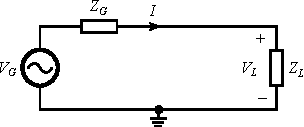
\includegraphics{img/analysis/generator_load}
    \caption{Equivalent circuit of a generator with given output impedance, $Z_G$, delivering power to a load of a given impedance, $Z_L$.}
    \label{fig:generator_load}
\end{figure}

To maximize the power transfered from a generator to a load, it is desired to have a reflection coefficient that is zero so that only forward waves are present on the transmission line. Figure~\ref{fig:generator_load} shows an equivalent circuit for this situation. The power in the load is found as \cite{pozar2011microwave}
\begin{equation}
    \label{eq:power1}
    P = \frac{1}{2} \real{V_LI^*} = \frac{1}{2} \real{\frac{|V_L|^2}{Z_L}}
    = \frac{1}{2} |V_L|^2 \real{\frac{1}{Z_L}}
\end{equation}
where
\begin{where}
\item[$P_L$] Power delivered to the load
\item[$V_L$] Voltage drop across the load
\item[$Z_L$] $R_L+jX_L$ is the load impedance
\item[$I$] Current through the load
\end{where}
Using basic circuit theory, (\ref{eq:power1}) can be expressed in terms of $V_G$ and $Z_G$, making it possible to derive the optimal $Z_G = R_G+jX_G$ for a fixed, complex load. Continuing from (\ref{eq:power1}),
\begin{equation}
    \begin{aligned}
        P &= \frac{1}{2} \left| V_G \frac{Z_L}{Z_L+Z_G} \right|^2 \real{\frac{1}{Z_L}} \\
        &= \frac{1}{2} |V_G|^2 \frac{|Z_L|^2}{|Z_L+Z_G|^2} \real{\frac{1}{Z_L}}\\
        &= \frac{|V_G|^2}{2} \frac{R_L^2+X_L^2}{(R_L+R_G)^2+(X_L+X_G)^2} \frac{R_L}{R_L^2 + X_L^2}\\
        &= \frac{|V_G|^2}{2} \frac{R_L}{(R_L+R_G)^2 + (X_L+X_G)^2}
    \end{aligned}
\end{equation}
The values of $R_G$ and $X_G$ that maximize the power delivered to the load, is found by 
\begin{enumerate}
\item Taking the partial derivative of $P$ with respect to $R_L$
\item Taking the partial derivative of $P$ with respect to $X_L$
\item Setting both of the above solutions equal to zero and solving for $R_G$ and $X_G$ (two equations with two unknowns)
    \begin{align}
        \dpd{P}{R_L} &= 0 \\
        \dpd{P}{X_L} &= 0
    \end{align}
\end{enumerate}
Doing so, yields the following solution,
\begin{equation}
    \begin{aligned}
        R_{G,\text{max}} &= R_L \\
        X_{G,\text{max}} &= -X_L
    \end{aligned}
\end{equation}
or $Z_{G,\text{max}} = Z^*_L$; the maximum power is transfered to the load when the generator impedance is the complex conjugate of the load impedance. In this situation the generator is said to be \emph{matched} to the load. Generally, the generator and the load would be connected through a transmission line with the characteristic impedance $Z_0$, so the maximum power transfer from generator to load will occur when both generator and load are matched to $Z_0$. 

% Mismatch loss, S11. |S11| = -6 dB  -->  SWR = 3

% Smith chart visualization

% Matching circuitry, L-network, smith chart ``ups and downs'', analytical formulas.

% Tuners: Series capacitor, shunt capacitor, variable inductor?

% Insertion loss, S21 for networks, equivalent series resistance, component Q.
